\section{Implementation and computational illustration}\label{sec:computation}

The experiments in this section test whether the predicted grid sizes appear
in practice and whether the certificates are cheap enough to check. They are
not a benchmark of competitive performance: the implementation is a reference
code in exact rational arithmetic, and all instance families with continuous
coordinates are synthetic (planted, random or constructed). The only library
instances we ran are binary (Section~\ref{sec:comp-limits}), so we do not test
whether modeled instances with continuous nonconvex terms have small width
and a moderate condition number. Appendix~\ref{app:computation} contains the
tables and details that this section summarizes.

\subsection{Implementation}\label{sec:comp-impl}
The reference implementation is written in Python with exact rational
arithmetic (Python's \texttt{fractions} module); floating-point input is
rejected. It handles explicit box QPs $\frac12x^\T Hx+b^\T x+c$ with continuous
and integer coordinates, supplied or heuristically computed (minimum-fill)
tree decompositions with arbitrary branching, and empty separators. It
implements the corrected grids of Section~\ref{sec:grids} with corrections
$\max\{H_{ii},0\}w^2/8$, the two-node grids $\{\ell_i,u_i\}$ for coordinates
with $H_{ii}\le0$, two-pass dynamic programming with all min-marginals,
filtering, and CT (Algorithm~\ref{alg:ct}) in the common-mesh form of
Lemma~\ref{lem:commonmesh}. It differs from the analysis in seven ways, none
of which affects validity (Appendix~\ref{app:computation} lists them); the
most important is that all coordinates share the mesh $h_j=s2^{-j}$, so the
analysis that applies is Lemma~\ref{lem:commonmesh} with the Euclidean
condition number $\kappa$, not Theorem~\ref{thm:approx}. Exact coordinate
descent from $\ell$, $u$ and the box midpoint provides the first incumbent
before stage~$0$, and each trial starts with the center at the current
incumbent.

Experiments E1--E3 below run single trials, that is, TRIAL
(Algorithm~\ref{alg:trial}) with the common mesh, a fixed grading~$\theta$
($\theta=0$ for uniform grids), no cap on the nodes per coordinate and a fixed
number of stages, in E1 also without filtering; the ``theorem'' grading is the
largest $2^{-\mu}$ with $8\kappa\theta^2\le1$ for the certified upper bound on
$\kappa$, which the algorithm itself does not know. Experiment E4 runs EX
(Algorithm~\ref{alg:ex}); the
default schedule of E2, experiments E5 and E6, the supplementary experiment
S1, the chain and the recourse runs use CT. In E2, E5, E6 and the chain no
trial was aborted by the cap: the only restarts occurred in E2, and each
followed a trial that reached its stage limit.

Certificates store the grids, the directed messages and the filtering
decisions of every stage, which is more than Theorem~\ref{thm:certificate}
requires. A separate checker recomputes every table and message, checks the
Bellman equalities, the min-marginals, every exclusion, the incumbent values
and the final status, and never calls the grid generator, the dynamic program
or the filtering code of the solver; it shares model parsing, decomposition
validation and objective evaluation with the solver. The checker is
independently written, not formally verified. On the runs of E1--E6, the
chain and the plain-grid recourse runs below with a solve time of at least
$0.1$ seconds, replay took between $0.81$ and $2.54$ times as long as the
solve. Code, inputs, raw results and reproduction scripts (one command per
experiment group), together with the solver files they import, are provided
as supplementary material.

All runs below used one thread per process and at most four processes on an
Intel Xeon w5-2565X under Windows Subsystem for Linux (WSL2) with
Python~3.13, on a machine shared with unrelated long-running jobs (load
average 11 to 19). Timings are single measurements and indicative only. Every
certificate on which a result in
Sections~\ref{sec:comp-growth}--\ref{sec:comp-recourse} rests was replayed by
its checker, and every replay was valid; the CT runs of S1 that only measure
when the gap falls below a threshold (Section~\ref{sec:comp-localized}) were
not replayed.

\subsection{Accuracy independence, conditioning and dimension}
\label{sec:comp-growth}
The planted family consists of nonconvex quadratics on $[-1,1]^n$ with Hessian
$H=2I+C$, where $C$ has path, random-tree or band sparsity. About a quarter of
the coordinates are at a bound at the planted minimizer $x^*$, all with a
strictly inward derivative of the same size; the other coordinates of $x^*$
are of the form $k/21$ with $\abs k\le10$, and on them the Hessian block
$H_{J_0J_0}$ has smallest eigenvalue $4/\kappa_{\mathrm{target}}$, up to a
rounding of the coupling scale to a multiple of $2^{-12}$. Entries of $C$ that
touch an active coordinate have size $2$ to $4$, and $H$ is indefinite in
every instance (its smallest eigenvalue is at most $-1.16$).
Parts~(a) and~(b) of Lemma~\ref{lem:growthcert} bracket $\kappa$ to within
$12\%$ (Appendix~\ref{app:computation}). The family is benign in
one respect: once $x^*$ is known, \eqref{eq:minorant} certifies it directly;
the grid solver does not use this. The minimizers are mostly off the grids:
over the runs of E1--E3 with $\kappa_{\mathrm{target}}\ge4$, 347 of 3{,}177
free coordinates of $x^*$, counted once per run ($11\%$), were nodes of the
last grid.

\begin{figure}[t]
\centering
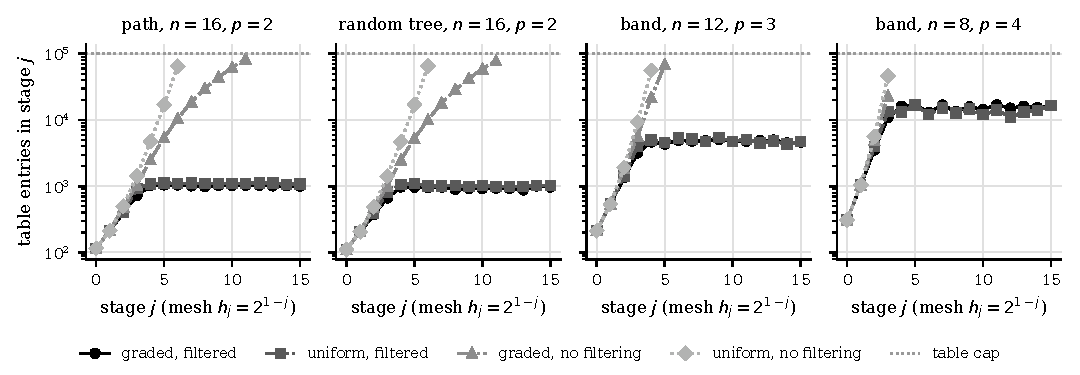
\includegraphics[width=\textwidth]{figures/E1_states_vs_stage.pdf}
\caption{Experiment E1: table entries per stage against the stage index $j$
(mesh $h_j=2^{1-j}$), median of three seeds, for graded and uniform grids with
and without filtering; $\theta=1/8$, $\kappa\in[3.99,4.45]$. A stage is plotted
only if all three runs completed it. Runs without filtering stop at the cap
of $10^5$ table entries per stage (dotted line).}\label{fig:E1}
\end{figure}

\paragraph{E1: accuracy.} Figure~\ref{fig:E1} shows the effect of filtering in
single trials with $\theta=1/8$. On the path with $n=16$, filtered graded
grids use about $1{,}000$ table entries per stage from stage~4 to stage~15,
while unfiltered graded grids reach $83{,}161$ entries at stage~11 and
unfiltered uniform grids $64{,}879$ at stage~6, after which both hit the cap.
Filtered uniform grids also plateau (about $1{,}100$ entries): filtering, not
the grading, removes the dependence on the accuracy. This is predicted by
(G1)--(G4) of Lemma~\ref{lem:commonmesh}, which also hold for $\theta=0$, so
the retained radius is still at most $4.2\sqrt{n\kappa}\,h_j$ and the next
uniform grid has at most $16.8\sqrt{n\kappa}+3$ nodes per continuous
coordinate. In all 876 stages of the filtered graded runs of E1 and the runs
of E2 and E3 with the theorem's grading (all with $8\kappa\theta^2\le1$), the
gap $D(y_j)$, the retained radius and the number of nodes per coordinate were
at most $0.28$, $0.18$ and $0.05$ times their bounds (G3)--(G5) in
Lemma~\ref{lem:commonmesh} (Appendix~\ref{app:computation}).

\begin{figure}[t]
\centering
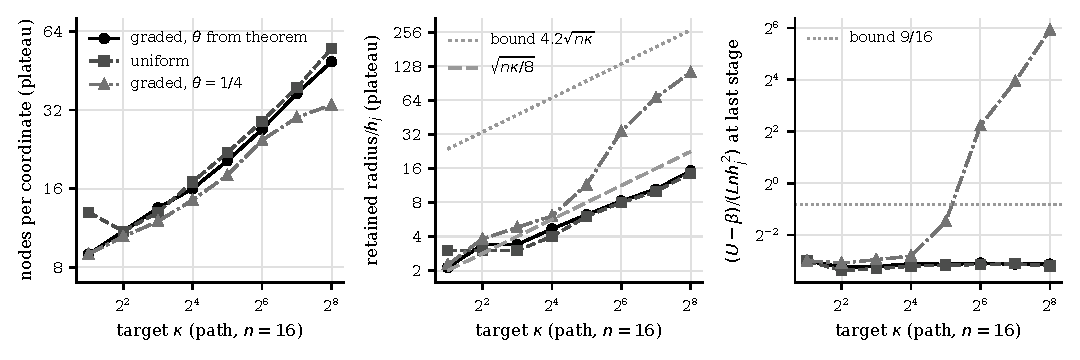
\includegraphics[width=\textwidth]{figures/E2_plateau_vs_kappa.pdf}
\caption{Experiment E2: path with $n=16$ and $\kappa_{\mathrm{target}}=
2,4,\dots,256$; the certified $\kappa$ lies in
$[0.97\,\kappa_{\mathrm{target}},1.12\,\kappa_{\mathrm{target}}]$. Left: nodes per
coordinate, the maximum over free coordinates and the median over the last
four stages and the three seeds. Middle: retained radius over $h_j$, same
statistics, with the bound $4.2\sqrt{n\kappa}$ of Lemma~\ref{lem:commonmesh}
and the reference $\sqrt{n\kappa/8}$, both evaluated at the lower end of the
certified $\kappa$ interval. Right: gap $U-\beta$ at the last stage over
$Lnh_j^2$, with the bound $9/16$.}
\label{fig:E2}
\end{figure}

\paragraph{E2 and E3: conditioning and dimension.} Figure~\ref{fig:E2} varies
$\kappa$ on the path with $n=16$, in single trials of 12 stages. With the
theorem's grading the plateau grows from 9 to 49 nodes per coordinate, and the
retained radius grows more slowly than $\sqrt\kappa$ and stays far below its
bound. With the fixed grading $\theta=1/4$ the condition
$8\kappa\theta^2\le1$ fails for every instance with
$\kappa_{\mathrm{target}}\ge4$; the trial still contracted for
$\kappa_{\mathrm{target}}\le32$, but for $\kappa_{\mathrm{target}}\ge64$ the
last-stage gap divided by $Lnh_j^2$ was $4.7$, $15$ and $61$. CT with
$\varepsilon=2^{-20}$ handled this automatically: it succeeded in its first
trial ($\theta=1/4$) for $\kappa_{\mathrm{target}}\le32$ and restarted once or
twice for larger $\kappa_{\mathrm{target}}$, earlier than
Lemma~\ref{lem:commonmesh} guarantees. For $\kappa_{\mathrm{target}}=2$ the
generator sets the couplings between free coordinates to zero
($H_{J_0J_0}=2I$); the free coordinates are then separable, and the initial
coordinate descent already returns~$x^*$. Experiment E3 varies $n$ on paths
with $n=4,8,\dots,128$ and $\kappa_{\mathrm{target}}=4$ ($\kappa\in[3.99,4.45]$),
in single trials of 11 stages. The plateau, measured as in
Figure~\ref{fig:E2} (left), grew from 7 to 26 nodes per free coordinate for filtered uniform grids, from 9
to 19 with the theorem's grading $\theta=1/8$, and from 9 to 17 with
$\theta=1/4$. This range of $n$ is too small to separate $\log n$ from
$\sqrt n$; Corollary~\ref{cor:uniformgrid} shows that uniform grids need order
$\sqrt{n\kappa}$ nodes on some instances.

\subsection{The expanding-box chain}\label{sec:comp-chain}
Table~\ref{tab:chain} in Appendix~\ref{app:computation} reports CT on the
family $\Psi_m$ of Proposition~\ref{lim:prop:messages}
(Example~\ref{ex:chain}) for $m=2,4,8,\dots,64$ and target gap $10^{-3}$.
The exact Bellman message for $\xi_m$ would need at least $2^{m-1}$
quadratic pieces, but the largest coordinate grid grows only from 5 to 11
nodes as $n$ grows from 4 to 128, and the number of stages grows linearly in
$m$, from 9 to 74, because the largest box width, $2^m-1$, enters the stage
count logarithmically. All runs succeeded in the first trial ($\theta=1/4$),
although $8\kappa\theta^2\le1$ fails: $\Psi_m=1$ at the point with $z_1=1$ and
all other coordinates~$0$, so every growth constant is at most $1$ and
$\kappa\ge10$. The minimizer $0$ is the lower corner of the box, the solver's
first descent start. Started at the upper corner instead, the runs used the
same numbers of stages, the same largest grid (except for $m=2$: 6 instead of
5 nodes) and between $2\%$ fewer and $8\%$ more table entries.

\subsection{Exact output and localized acceptance}\label{sec:comp-exact}
Experiment E4 ran EX on twenty small instances: twelve random unplanted
mixed-integer QPs ($n=3,\dots,6$, one or two integer coordinates), three with
two isolated minimizers, three planted instances ($n=6$) and two with segments
of minimizers, with limits of 3{,}000 stages and 30 seconds (5 seconds for the
last two). An independent enumeration of integer assignments and continuous
faces gives the reference optima. Exact output was certified for 18
instances, all with the correct value and an optimal point. Three of them
($n=3$) have no continuous coordinate with positive curvature and needed at
most one stage. Because our implementation of EX starts at $q=4$, doubles $q$
after each round and restarts the grid solver in every round,
the number of stages of the other 15 is close to the precision $q$ of the
last round, a power of two near the required number of bits
$\log_2(\Omega'W)$, where $W$ is the denominator of the optimal value and
$\Omega'\ge\Omega$ the implementation's height constant: 67 to 534 stages for
49 to 342 bits (Appendix~\ref{app:computation}); with $\Omega'=\Omega$
from~\eqref{eq:exact-constants}, 21 to 315 bits would suffice. The two instances with
segments of minimizers stopped at the time limit with certified gaps of about
$2^{-11}$, against about $2^{-53}$ required. They have set growth
(Remark~\ref{rem:setgrowth}) but no point growth, so Theorem~\ref{thm:exact}
guarantees only termination; their objective contains $a(x_0-x_1)^2$, a
multiple of the instance of Proposition~\ref{lim:prop:setgrowth} with $n=2$,
on which every CT run that certifies accuracy $\varepsilon$ ends with at least
$1+1/(2\sqrt\varepsilon)$ nodes per coordinate.

\paragraph{S1: localized acceptance.}\label{sec:comp-localized}
The supplementary experiment S1 tests the localized acceptance rule of
Proposition~\ref{prop:local} on 30 further random instances generated as in
E4, with $n=4,6,8,12,16$. After every stage of one replayed CT run with
$\varepsilon=2^{-60}$, the test was applied to the face candidate of
Definition~\ref{def:facecand}, which Corollary~\ref{cor:local} covers, and to
the stationary point of the face of the stage incumbent. Both accepted the
same 29 instances, the face candidate within nine stages and the incumbent
rule within five; on 12 of them the incumbent rule passes even with $X$ in
place of the narrowed box, that is, without the filtering history. The
accepted values agreed with those of EX on all 29 instances, and on the 12
instances with $n\le6$ also with the enumeration. The one failure has two
optimal vertices that differ in a concave coordinate, a tie outside the scope
of Corollary~\ref{cor:local}. EX, as implemented, used up to 542 stages on
these instances. An optimal candidate passes the test of
Proposition~\ref{prop:accept} once the certified gap is below $1/(\Omega'W)$;
on the five instances on which EX used the most stages, one CT run reached
this threshold after 40 to 72 stages with $\Omega'=\Omega$ and 139 to 157
with the implementation's constant.

\subsection{Comparison with a global solver}\label{sec:comp-scip}
Experiment E5 compares CT with SCIP~10.0
\cite{VigerskeGleixner2018,HojnyEtAl2025} on 21 planted instances with
$\kappa_{\mathrm{target}}=4$ ($\kappa\in[3.99,4.45]$), with $n=8$ to $128$ and
bag sizes 2 to 4. SCIP ran single-threaded on the epigraph formulation $\min\{t:t\ge F(x)\}$, with the coefficients rounded to
double precision, absolute gap $10^{-6}$ and a 20-second limit. CT used
$\varepsilon=10^{-6}$ and a 60-second limit; it reached a replayed gap below
$10^{-6}$ on all 21 instances in its first trial, in at most $6.9$ seconds.
SCIP reported its gap as reached on the 12 instances with $n\le16$ and stopped
at the time limit on all nine paths with $n\ge32$ (Table~\ref{tab:scip} in
Appendix~\ref{app:computation}). Its dual bounds were valid, but its reported
interval did not contain the optimum in any run: every reported primal bound
lay below the optimum, by $1.8\cdot10^{-6}$ to $1.6\cdot10^{-5}$. SCIP's
incumbents lay slightly outside the box: every coordinate that is at a bound
in $x^*$ violated that bound by about $10^{-8}$, which SCIP's feasibility
tolerance permits. Moving such a coordinate outward decreases $F$ at the rate
of its inward derivative, and these violations account for $51\%$ to $94\%$
of the shortfall; a violation of the epigraph constraint by $9\cdot10^{-7}$
accounts for the rest. Projected onto the box, the incumbents were optimal to within
$1.3\cdot10^{-14}$, and on the instances with $n\le16$ their exact gap to the
dual bound was $2.8\cdot10^{-6}$ to $6.8\cdot10^{-6}$, so the requested
$10^{-6}$ was not reached. This is the usual behavior of floating-point
solvers, and rigorous bounds need safe computations
\cite{NeumaierShcherbina2004} or an exact check. A longer time limit, tighter
tolerances or an objective offset did not change these outcomes
(Appendix~\ref{app:computation}). The comparison uses one formulation, default
settings and a family that favors decompositions of small width; it is not a
performance ranking.

\subsection{Random instances without planted structure}\label{sec:comp-random}
Experiment E6 uses 40 unplanted random continuous box QPs on $[-1,1]^n$ with
path or band sparsity (bag sizes 2 and 3), $n=8,12,16,24$ and five seeds
each. All Hessians are indefinite, and nothing about the minimizer or the
conditioning is prescribed. CT was run at
$\varepsilon=2^{-10},2^{-20},\dots,2^{-50}$ and reached every target in its
first trial ($\theta=1/4$). The largest grid had 8 to 18 nodes per coordinate.
From $\varepsilon=2^{-10}$ to $2^{-50}$ it stayed the same on 27 of the 40
instances and changed by at most 5 nodes on the others, while the number of
stages grew linearly in $\log(1/\varepsilon)$, from 7--9 to 27--29
(Table~\ref{tab:random} in Appendix~\ref{app:computation}). At the
stationary point $\hat x$ of the face of the final incumbent,
Lemma~\ref{lem:growthcert}(a) certified point growth on 11 instances, with
certified $\kappa\ge4.5$; there $8\kappa\theta^2>1$ for $\theta=1/4$, so the
first trial succeeded although Lemma~\ref{lem:commonmesh} does not guarantee
it. On the other 29 instances growth and $\kappa$ remain unknown; on 28 of
them the localized test of Proposition~\ref{prop:local} proved a candidate
optimal, and on the remaining one no candidate was proved optimal. For $n=8$
all candidates
agree with the enumeration.

\subsection{Recourse}\label{sec:comp-recourse}
Six designed instances compare plain corrected grids (CT) with the recourse
pipeline at target gap $2^{-10}$ and a 20-second limit
(Table~\ref{tab:recourse} in Appendix~\ref{app:computation}). On two affine
stars ($n=5$ and $17$), recognition of the globally affine responses and an
exact solve of the reduced problem took at most $0.07$ seconds, while plain
grids stopped at the time limit with gaps $0.019$ and $1.23$. On the
piecewise instances $\phi_M-z^2$ of Example~\ref{ex:cv-fm}, the certified
convex value factor removed the dependence on $M$, whereas plain grids needed
498 table entries for $M=1$ and $35{,}600$ for $M=100$. On a dense instance
with $n=33$ whose residual is concave in each coordinate and submodular, the
minimum-cut oracle of Section~\ref{sec:cuts} certified the target gap in
$0.08$ seconds; plain grids, with a decomposition of bag size 33, stopped at
the table limit before the first stage. All certificates were replayed; the
checkers of the recourse pipeline reuse the solver's grid, table and lifting
code and are therefore not independent in the sense of
Section~\ref{sec:comp-impl}. These are designed examples of the structures in
Section~\ref{sec:recourse}, not hard instances.

\subsection{Limits}\label{sec:comp-limits}
The cost of the method is exponential in the bag size, and exact rational
arithmetic dominates the running time; the band with bag size four already
takes several seconds. On two binary QPLIB instances \cite{FuriniEtAl2019}
the first grid is exact, so the method is plain dynamic programming over the
decomposition. QPLIB\_3852 (231 variables, minimum-fill bag size 20) was
solved exactly in one stage, with $5.7\cdot10^6$ table entries, 156 seconds
and 4.4\,GB of memory; the certified bounds coincide at $-234$, the library's
value after the sign change to minimization. We did not replay this
certificate, because the reference checker is too slow at this size. For
QPLIB\_5881 (120 variables, bag size 94) the first stage would need about
$8\cdot10^{28}$ table entries. Large width, not the accuracy, is the binding
limit; Section~\ref{sec:limits} shows that this is unavoidable in the worst
case.
